\chapter{一般概率模型与随机对象}
\label{chap:probability-models}

掷两枚骰子，三位记录员各自记下结果：第一位写下两枚骰子的点数，第二位只写点数和，第三位只写点数和是奇是偶。
三份记录来自同一次试验，能回答的问题却不同：只有第一位能判断“第一枚掷出$6$”是否发生，第三位甚至分不清点数和是$7$还是$9$。
再看一个排队的例子：顾客有$40\%$的机会到达时窗口空闲、等待时间恰好为$0$，其余时候等待时间服从指数分布。
这个等待时间既没有概率表，也没有普通密度，它的平均值该怎么算？
还有一个更隐蔽的问题：两个量的概率规律完全相同，它们是否就是“同一个随机变量”？两个量各自的规律都已知，它们一起出现的规律是否也就确定了？

卷一处理概率问题时，计算都落在两种形式上：列出概率表逐项相加，或者写出密度再积分。
上面几个问题说明，这两种形式背后还有几件事没有分开：试验结果本身、我们允许判断的事件、观测到的数值，以及数值的概率规律。
第~\ref{chap:measure-spaces}章已经建立了可测空间、测度、推前和一般积分，本章用这些工具把上述几层分开，使计算不再依赖概率表或密度。

全章沿“结果—观测—规律—累计”的顺序展开。
第~\ref{sec:pmod-probability-space}节把概率模型写成概率空间，并说明零概率事件与“几乎必然”的含义；第~\ref{sec:pmod-random-objects}节把观测写成可测映射，用它生成的$\sigma$代数描述观测带来的信息。
有了观测，第~\ref{sec:pmod-distributions}节把概率从样本空间搬到取值空间，得到分布，并区分“同分布”“几乎处处相等”与联合分布；第~\ref{sec:pmod-independence}节研究联合分布何时分解成各自分布的乘积，这就是独立性。
第~\ref{sec:pmod-expectation}节把求和与密度积分统一成对概率测度的积分，讨论矩条件和几个基本不等式，它们是后面三章研究条件期望和收敛时反复使用的工具。

\section{概率空间}
\label{sec:pmod-probability-space}

一个概率模型不能只列出可能结果。
同一次试验可以按不同精细程度记录，我们必须同时说清：哪些结果可能出现，哪些关于结果的问题允许回答，这些问题的答案各有多大概率。
本节先把这三件事写成概率空间，再处理概率为零的事件。

\subsection{事件与概率模型}

\paragraph{概率模型的三个组成部分}
卷一用样本空间、事件和概率描述随机试验，并要求概率满足非负、总和为$1$与可数可加。
第~\ref{chap:measure-spaces}章的可测空间正好给出“哪些集合允许测量”，测度给出“这些集合各有多大”。
概率模型就是总质量为$1$的测度空间。

\begin{definition}[概率空间]
\label{def:pmod-probability-space}
设$\Omega$是非空集合，$\mathcal F$是$\Omega$上的$\sigma$代数，$\mathbb P:\mathcal F\to[0,1]$是$(\Omega,\mathcal F)$上的测度，并且$\mathbb P(\Omega)=1$。
称三元组$(\Omega,\mathcal F,\mathbb P)$为\term{概率空间}（probability space），称$\Omega$为样本空间，$\mathcal F$中的集合为\term{事件}（event），$\mathbb P$为概率测度。
\end{definition}

定义中$\mathcal F$不能省略。
只有属于$\mathcal F$的集合才有概率，一个$\Omega$的子集若不在$\mathcal F$中，模型就不对它作出任何概率判断。
概率的基本运算规则都直接由测度的性质得到：补事件满足$\mathbb P(\Omega\setminus A)=1-\mathbb P(A)$，$A\subseteq B$时$\mathbb P(A)\le\mathbb P(B)$，任意一列事件满足
\[
  \mathbb P\Bigl(\bigcup_{n=1}^\infty A_n\Bigr)\le\sum_{n=1}^\infty\mathbb P(A_n).
\]
由于总质量有限，事件单调增加或单调减少时，概率都随之收敛到极限事件的概率。
这些结论在第~\ref{chap:measure-spaces}章已经对一般测度成立，这里不再重证；Lebesgue测度的构造也不在本章重复。

\paragraph{同一试验的三种记录}
回到章首的两枚骰子。
样本空间取有序对$\Omega=\{1,\dots,6\}^2$，$36$个结果等可能。
三位记录员保留的信息不同，可以用三个$\sigma$代数表示。

\begin{example}[两枚骰子的三种观测]
\label{ex:pmod-dice-records}
记$\omega=(i,j)$，点数和$S(\omega)=i+j$。
完整记录对应$\mathcal F_{\mathrm{full}}=\mathcal P(\Omega)$，$36$个单点都可以单独判断，共有$2^{36}$个事件。
只记录点数和时，能判断的事件恰好是若干个$\{S=s\}$（$s=2,\dots,12$）的并，记这一族为$\mathcal F_{\mathrm{sum}}$，它有$11$个不可再分的块，共$2^{11}$个事件。
只记录奇偶时，能判断的事件只有
\[
  \mathcal F_{\mathrm{par}}=\bigl\{\varnothing,\ \{S\text{为偶数}\},\ \{S\text{为奇数}\},\ \Omega\bigr\}.
\]
三族满足$\mathcal F_{\mathrm{par}}\subseteq\mathcal F_{\mathrm{sum}}\subseteq\mathcal F_{\mathrm{full}}$。
事件$\{S=7\}$由$(1,6),(2,5),\dots,(6,1)$六个结果组成，属于$\mathcal F_{\mathrm{sum}}$，概率为$6/36=1/6$；它不属于$\mathcal F_{\mathrm{par}}$，因为它只是偶数和奇数两个块之一的一部分。
事件“第一枚掷出$6$”包含$(6,1)$却不包含与之同和的$(1,6)$，不是若干$\{S=s\}$的并，所以不属于$\mathcal F_{\mathrm{sum}}$。
\end{example}

图~\ref{fig:pmod-dice-information}把三种记录画在同一个$6\times6$网格上：(b)中同一条反对角线上的格子构成一个不可再分的块，(c)中同色格子构成一块。
记录越粗，块越大，能回答的问题越少；但三种记录用的是同一个$\Omega$和同一组等可能的结果。
在较粗的$\sigma$代数上，概率只是原来$\mathbb P$的限制，例如$(\Omega,\mathcal F_{\mathrm{sum}},\mathbb P|_{\mathcal F_{\mathrm{sum}}})$仍是概率空间。
因此写一个概率模型时，$\mathcal F$说明了“允许问什么”，它和$\Omega$一样是模型的一部分。

\begin{figure*}[htbp]
  \centering
  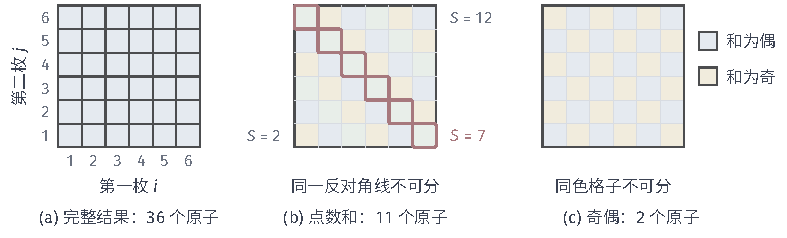
\includegraphics[width=133mm]{figures/02-abstract-mathematics/02-probability-spaces/tikz/pmod-dice-information/figure.pdf}
  \caption{两枚公平骰子的三种记录。格子$(i,j)$表示第一枚$i$点、第二枚$j$点，$36$格等可能。(a) 完整记录，每格单独可辨；(b) 只记录点数和$S$，同一条反对角线上的格子同色、不可区分，共$11$块（图中称原子），红框为$\{S=7\}$；(c) 只记录$S$的奇偶，只剩两块。颜色只区分相邻的块，不表示概率大小。}
  \label{fig:pmod-dice-information}
\end{figure*}

\paragraph{不必有密度的概率测度}
卷一的概率模型大多由概率表或普通密度给出。
在实轴的Borel结构上，这两类分别是点质量的可数混合$\sum_kp_k\delta_{x_k}$，以及形如$A\mapsto\int_Af(x)\,dx$的测度。
第~\ref{sec:measure-same-space-comparison}节的Lebesgue分解说明，实轴上的任何概率测度都可以写成相对长度绝对连续的部分与奇异部分之和；奇异部分可以含点质量，也可以不含任何点质量。

后一种情况的典型例子是\term{Cantor分布}（Cantor distribution）。
把三进制展开中每一位独立、等可能地取$0$或$2$，得到$[0,1]$中的随机点（这样的独立数字可以在$[0,1)$均匀模型上实现，见第~\ref{sec:pmod-independence}节的例~\ref{ex:pmod-binary-digits}）。
前$n$位数字的$2^n$种取法对应$2^n$个互不相交、长度为$3^{-n}$的闭区间，随机点落在哪个区间由前$n$位数字决定，概率为$2^{-n}$。任一单点至多属于其中一个区间，所以它的概率不超过$2^{-n}$；这对一切$n$成立，因而为零。
同时全部质量落在$2^n$个这样的区间之并中，总长度$(2/3)^n\to0$。
这个分布既没有概率表，也没有相对长度的密度。
章首的等待时间则是点质量与密度部分的混合。
本部分直接以测度$\mathbb P$为对象作计算，不要求它属于某种表示；常见分布族的系统整理放在\BookPartRef{part:probability-distributions}{卷四“概率分布”部分}。

\subsection{零概率事件与几乎必然}

\paragraph{零概率不等于不可能}
在$[0,1]$上取Borel$\sigma$代数与长度，得到\emph{$[0,1]$均匀模型}；令$X(\omega)=\omega$。
对任意固定的$x\in[0,1]$和$h>0$，事件$\{X=x\}$包含于$\{x-h\le X\le x+h\}$，后者的概率不超过$2h$。
令$h\to0$，得$\mathbb P(X=x)=0$。
可是$\{X=x\}=\{x\}$并不是空集：结果恰好是$x$完全可能发生，每次试验中$X$也总要取到$[0,1]$中的某个值。这个非空事件的概率却为零。

概率为零的事件称为\term{零概率事件}（null event），它必须和空事件分开。
空事件在任何概率测度下都不发生；零概率事件可以发生，只是在模型的累计意义下不占质量。
零概率也总是相对于具体的$\mathbb P$而言：在点质量$\delta_x$下，单点$\{x\}$的概率是$1$。

\paragraph{几乎必然的定义}
很多结论在个别结果上失败，但失败的结果合起来没有概率。
第~\ref{chap:measure-spaces}章称这样的性质“几乎处处”成立；在概率空间上习惯说“几乎必然”。

\begin{definition}[几乎必然]
\label{def:pmod-almost-sure}
设$(\Omega,\mathcal F,\mathbb P)$是概率空间，$\mathcal Q$是关于样本点$\omega$的一个命题。
若存在事件$N\in\mathcal F$，$\mathbb P(N)=0$，使得每个$\omega\notin N$都满足$\mathcal Q$，就称$\mathcal Q$\term{几乎必然}（almost surely）成立，简记为a.s.。
等价地，存在概率为$1$的事件，在其上$\mathcal Q$处处成立。
\end{definition}

定义只要求失败的结果被某个零概率事件盖住，不要求失败集合本身是事件。
这一区别在下文讨论完备化时会用到。

\begin{example}[只在一点失败的极限]
\label{ex:pmod-power-limit}
在$[0,1]$均匀模型上令$X_n(\omega)=\omega^n$。
当$0\le\omega<1$时$\omega^n\to0$；当$\omega=1$时$X_n(1)=1$对一切$n$成立。
取$N=\{1\}$，$\mathbb P(N)=0$，在$N$之外$X_n\to0$，所以$X_n\to0$几乎必然成立。
它不是处处成立的：在$\omega=1$这个结果上，极限是$1$。
\end{example}

图~\ref{fig:pmod-almost-sure-limit}画出了几条$\omega\mapsto\omega^n$。
$n$越大，曲线越早贴近$0$，只在右端急剧抬升到$1$；逐点极限是除右端点外恒为零的函数。
抬升的区域越来越窄，但对每个固定的$n$都存在；真正的例外只剩一点，它不占概率。

\begin{figure}[htbp]
  \centering
  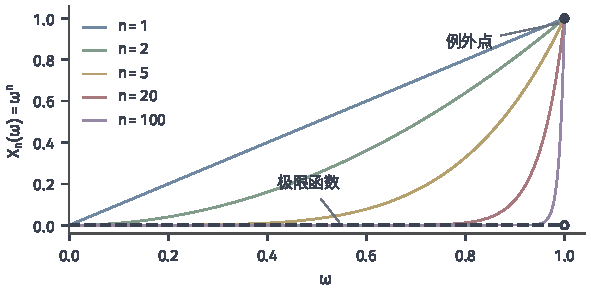
\includegraphics[width=100mm]{figures/02-abstract-mathematics/02-probability-spaces/matplotlib/pmod-almost-sure-limit/figure.pdf}
  \caption{$[0,1]$均匀模型上的$X_n(\omega)=\omega^n$，$n=1,2,5,20,100$。虚线是逐点极限：$\omega<1$时为$0$，$\omega=1$时为$1$（实心点）。例外集合$\{1\}$的概率为零，所以$X_n\to0$几乎必然成立，但不是处处成立。}
  \label{fig:pmod-almost-sure-limit}
\end{figure}

\paragraph{例外集合的合并与量词}
设一列命题$\mathcal Q_1,\mathcal Q_2,\dots$各自几乎必然成立，例外分别被零概率事件$N_1,N_2,\dots$盖住。
取$N=\bigcup_kN_k$，由可数次可加性
\[
  \mathbb P(N)\le\sum_{k=1}^\infty\mathbb P(N_k)=0,
\]
而在$N$之外所有$\mathcal Q_k$同时成立。
所以“对每个$k$几乎必然成立”可以升级为“几乎必然对所有$k$同时成立”：可数多个例外可以并入一个共同的零概率事件。

不可数多个例外没有这个保证。
在$[0,1]$均匀模型中，对每个固定的$x$，“$X\ne x$”几乎必然成立，因为例外集合$\{x\}$的概率为零。
但“对所有$x\in[0,1]$都有$X\ne x$”在任何结果上都不成立：所有单点的并就是整个$\Omega$。
因此遇到“对所有$t$”这类量词时，先数清$t$的范围：可数时直接合并例外；不可数时需要连续性或可分性等额外结构，把问题化为可数个时刻。
后面讨论随机变量列的收敛时，指标$n$只取可数个值，这正是可以直接合并例外的情形。

\paragraph{零概率集合上的改动}
“几乎必然”允许我们在零概率集合上忽略差异，但改动一个随机变量时还要核对可测性。
设$N\in\mathcal F$，$\mathbb P(N)=0$，$S\subseteq N$，把可测函数$X$在$S$上改成别的值得到$Y$。
若$S$本身不在$\mathcal F$中，$\{Y\in B\}$可能包含$S$的某个不可测部分，于是$Y$不一定可测。

有两种处理方式。
一是改用完备化的概率空间$(\Omega,\overline{\mathcal F},\overline{\mathbb P})$：把零概率事件的全部子集补进事件范围，原有事件的概率不变，此时零概率集合上的任意改动都保持可测（完备化的构造见第~\ref{sec:measure-general-structure}节）。
二是只在可测的零概率事件上、以可测的方式改动，例如把$X$在$N$上改成$0$。
本部分说两个随机变量“几乎必然相等”时，两者都假定是可测的；所谓选取一个“版本”，指在几乎必然相等的可测函数中选一个代表，所有概率与期望都不依赖这一选择。

\section{随机对象与观测信息}
\label{sec:pmod-random-objects}

固定概率空间之后，我们关心的通常不是$\omega$本身，而是对它的某种观测：骰子点数和、等待时长、一个特征向量或一张网络。
本节先说明一个观测需要满足什么条件，才能对“观测值落在某处”谈概率；再说明一个观测让我们能分辨哪些事件。

\subsection{随机对象的可测性}

\paragraph{可测映射与可问的事件}
设观测把每个结果$\omega$送到某个取值空间中的点$X(\omega)$。
我们想问的是$\mathbb P(X\in B)$，即结果集合
\[
  \{X\in B\}=\{\omega\in\Omega:X(\omega)\in B\}=X^{-1}(B)
\]
的概率。
这要求$X^{-1}(B)$属于$\mathcal F$，否则概率根本没有定义。
取值空间同样要先规定哪些集合$B$可以问，于是它也是一个可测空间。

\begin{definition}[随机对象]
\label{def:pmod-random-object}
设$(\Omega,\mathcal F,\mathbb P)$是概率空间，$(E,\mathcal E)$是可测空间。
若映射$X:\Omega\to E$对每个$B\in\mathcal E$都满足$X^{-1}(B)\in\mathcal F$，就称$X$是取值于$(E,\mathcal E)$的\term{随机对象}（random element）。
取值于$(\mathbb R,\mathcal B(\mathbb R))$的随机对象称为\term{随机变量}（random variable），取值于$(\mathbb R^d,\mathcal B(\mathbb R^d))$的称为$d$维\term{随机向量}（random vector）。
\end{definition}

换句话说，随机对象就是从$(\Omega,\mathcal F)$到$(E,\mathcal E)$的可测映射，“随机”只来自$\omega$的不确定，映射本身是确定的。
图~\ref{fig:pmod-preimage}画出了这一关系：取值空间中的集合$B$被拉回为样本空间中的事件$\{X\in B\}$，后者可以由不相连的几块组成，只要它属于$\mathcal F$就有概率。
注意记号$X^{-1}(B)$只表示原像，并不要求$X$可逆。

\begin{figure*}[htbp]
  \centering
  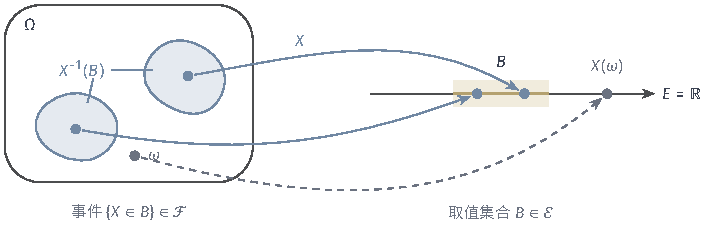
\includegraphics[width=120mm]{figures/02-abstract-mathematics/02-probability-spaces/tikz/pmod-preimage/figure.pdf}
  \caption{随机对象$X$是从样本空间$\Omega$到取值空间$E$的映射。取值集合$B$（右侧黄色区间）的原像$X^{-1}(B)=\{X\in B\}$是$\Omega$中的蓝色区域，可以分成不相连的几块；落在区域外的$\omega$被送到$B$之外。可测性要求每个$B\in\mathcal E$的原像都是事件。示意图，不含数值。}
  \label{fig:pmod-preimage}
\end{figure*}

\paragraph{常见的取值空间}
取值空间的可测结构要按问题选定，然后才能核对“哪些问题是事件”。
实值观测用实轴的Borel结构，有限维向量用$\mathbb R^d$的Borel结构；由第~\ref{chap:measure-spaces}章，$\mathcal B(\mathbb R^d)$与$d$个$\mathcal B(\mathbb R)$的乘积$\sigma$代数相同。
$m\times n$的\term{随机矩阵}（random matrix）把$\mathbb R^{m\times n}$按元素等同于$\mathbb R^{mn}$，沿用其Borel结构。
需要允许$\pm\infty$时（例如一列随机变量的上确界），取扩充实轴$[-\infty,+\infty]$，其可测集是形如$B\cup D$的集合，其中$B\in\mathcal B(\mathbb R)$，$D\subseteq\{-\infty,+\infty\}$。

离散的结构对象也可以作为取值空间。
固定顶点集$V=\{1,\dots,n\}$，所有简单无向图组成有限集$\mathcal G_n$，共有$2^{n(n-1)/2}$个元素，取其幂集为可测结构。
一个随机简单图$G:\Omega\to\mathcal G_n$可测，当且仅当每个$\{G=g\}$都是事件；这又等价于每条边的指示$\mathbb I_{\{\{i,j\}\in G\}}$都是随机变量。
前一个方向成立，是因为“边$\{i,j\}$出现”是有限个$\{G=g\}$的并；后一个方向成立，是因为$\{G=g\}$是有限个“某边出现”或“某边不出现”的交。
由于$\mathcal G_n$的每个子集都可测，“$G$连通”“$G$含三角形”这类问题在$G$可测时自动是事件。

\paragraph{用生成族检查可测性}
逐个检查$\mathcal E$中所有集合的原像通常做不到，好在取原像与补集、可数并可以交换。
若$\mathcal E$由集合族$\mathcal C$生成，则满足$X^{-1}(B)\in\mathcal F$的$B$构成一个$\sigma$代数，只要它包含$\mathcal C$就包含整个$\mathcal E$。
于是对实值$X$，只需检查$\{X\le a\}\in\mathcal F$对每个实数$a$（甚至每个有理数$a$）成立。

对$\bm X=(X_1,\dots,X_d)$，$\bm X$是随机向量当且仅当每个坐标$X_i$都是随机变量。
若$\bm X$可测，坐标投影连续因而Borel可测，$X_i$是可测映射的复合，仍可测；反过来，若每个$X_i$可测，则
\[
  \{\bm X\in(-\infty,a_1]\times\cdots\times(-\infty,a_d]\}=\bigcap_{i=1}^d\{X_i\le a_i\}\in\mathcal F,
\]
而这类左下象限生成$\mathcal B(\mathbb R^d)$。
复合保持可测：若$g:(E,\mathcal E)\to(E',\mathcal E')$可测，则$(g\circ X)^{-1}(C)=X^{-1}(g^{-1}(C))$，所以$g(X)$也是随机对象。
据此，$X+Y$、$XY$、$\max\{X,Y\}$、$|X|^p$都是随机变量，因为它们是随机向量$(X,Y)$的连续函数；一列随机变量的$\sup_n$、$\liminf_n$、$\limsup_n$是扩充实值随机变量，因为它们只涉及可数次运算。

可测性只保证所问的事件有概率，不提供更多性质。
它不意味着$X$关于$\omega$连续（$\Omega$上甚至可以没有拓扑），不意味着$X$与其他观测独立，也不意味着$X$的期望有限。
取值为整条曲线或整个函数时，选择什么可测结构取决于要问哪些问题，这在第~\ref{part:function-spaces}部分和\BookPartRef{part:dynamical-systems-control-decision-and-games}{卷三“过程与轨迹演化”部分}按用途建立，本章只处理有限维与一般可测取值对象的共同结构。

\subsection{随机对象生成的信息}

\paragraph{观测能分辨哪些事件}
只看到骰子点数和$S$的记录员，能判断的恰好是形如$\{S\in B\}$的事件：知道$S(\omega)$以后，就知道$\omega$是否落在其中。
一般观测也是如此。

\begin{definition}[随机对象生成的$\sigma$代数]
\label{def:pmod-generated-sigma}
设$X$是取值于$(E,\mathcal E)$的随机对象。称
\[
  \sigma(X)=\{X^{-1}(B):B\in\mathcal E\}
\]
为$X$生成的$\sigma$代数。
\end{definition}

由于取原像与补集、可数并交换，$\sigma(X)$确实是$\sigma$代数；由$X$的可测性，$\sigma(X)\subseteq\mathcal F$。
任何使$X$可测的$\sigma$代数$\mathcal G$都必须包含全部$X^{-1}(B)$，所以$\sigma(X)$是$\Omega$上使$X$可测的最小$\sigma$代数。
它的含义是：一个事件$A$属于$\sigma(X)$，当且仅当它可以写成$\{X\in B\}$的形式，于是知道$X(\omega)$就能判断$\omega$是否属于$A$。
在例~\ref{ex:pmod-dice-records}中，$\sigma(S)=\mathcal F_{\mathrm{sum}}$，而奇偶记录生成的正是$\mathcal F_{\mathrm{par}}$。

\paragraph{变换只会减少信息}
对观测作进一步加工，只能丢掉信息，不能凭空增加。
设$g:(E,\mathcal E)\to(E',\mathcal E')$可测，$Y=g(X)$。对每个$C\in\mathcal E'$，
\[
  Y^{-1}(C)=X^{-1}\bigl(g^{-1}(C)\bigr)\in\sigma(X),
\]
所以
\begin{equation}
  \sigma(g(X))\subseteq\sigma(X).
  \label{eq:pmod-function-information}
\end{equation}
信息减少因此有了精确的意思：$g(X)$能判断的事件是$X$能判断的事件的一部分。
若$g$是双射且逆映射也可测，上式两边相等，可逆的重新编码不改变信息。

\begin{example}[区间上的两级观测]
\label{ex:pmod-interval-information}
在$[0,1)$上取Borel$\sigma$代数与长度，令$X(\omega)=\lfloor4\omega\rfloor$，$Y=\lfloor X/2\rfloor=\lfloor2\omega\rfloor$。
$X$取$0,1,2,3$，把$\Omega$分成四个长$1/4$的区间；$\sigma(X)$由这些区间的并组成，共$2^4=16$个事件。
$Y$只取$0,1$，$\sigma(Y)=\{\varnothing,[0,1/2),[1/2,1),\Omega\}$。
事件$\{X=1\}=[1/4,1/2)$属于$\sigma(X)$，却只是$\{Y=0\}$的一半，所以不属于$\sigma(Y)$：知道$Y=0$并不能判断$X$是否为$1$。
\end{example}

图~\ref{fig:pmod-generated-partitions}把两级观测上下对齐（图中把不可再分的块称为原子）。
上一行的每个块都完整地落在下一行的某个块里，这就是式~\eqref{eq:pmod-function-information}的图形含义；反过来，下一行的块不能拆开，红框中的事件对$Y$不可见。
对取有限个值的观测（取值空间中单点可测），$\sigma(X)$总是由它的等值块的并组成，信息的多少就是划分的粗细。
反过来的问题——若$\sigma(Y)\subseteq\sigma(X)$，$Y$是否一定是$X$的函数——由第~\ref{chap:conditional-expectation}章的Doob--Dynkin引理（定理~\ref{thm:cond-doob-dynkin}）给出肯定回答。

\begin{figure*}[htbp]
  \centering
  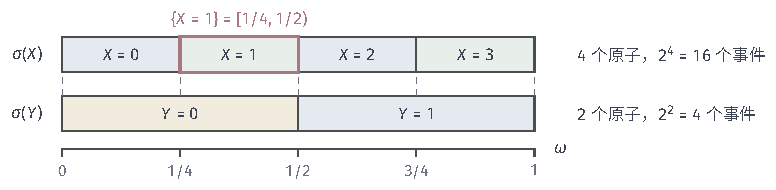
\includegraphics[width=131mm]{figures/02-abstract-mathematics/02-probability-spaces/tikz/pmod-generated-partitions/figure.pdf}
  \caption{$[0,1)$均匀模型上的两级观测。上行$X=\lfloor4\omega\rfloor$把区间分成四块，生成$16$个事件；下行$Y=\lfloor X/2\rfloor$只分成两块，生成$4$个事件。虚线表明$X$的每一块都落在$Y$的某一块内；红框中的$\{X=1\}$属于$\sigma(X)$而不属于$\sigma(Y)$。}
  \label{fig:pmod-generated-partitions}
\end{figure*}

\paragraph{多个观测的共同信息}
同时看到有限个观测$X_1,\dots,X_m$时，把它们合成一个映射$(X_1,\dots,X_m)$，取值于乘积空间$E_1\times\cdots\times E_m$，其可测结构为乘积$\sigma$代数$\mathcal E_1\otimes\cdots\otimes\mathcal E_m$。
矩形的原像是
\[
  \{(X_1,\dots,X_m)\in B_1\times\cdots\times B_m\}=\bigcap_{i=1}^m\{X_i\in B_i\},
\]
它属于$\mathcal F$；矩形生成乘积$\sigma$代数，所以合成映射可测。
记$\sigma(X_1,\dots,X_m)=\sigma\bigl((X_1,\dots,X_m)\bigr)$。

这个$\sigma$代数恰好是包含$\sigma(X_1)\cup\cdots\cup\sigma(X_m)$的最小$\sigma$代数，也就是“把各个观测的信息合起来”。一方面，$X_i$是合成映射与坐标投影的复合，所以每个$\sigma(X_i)$都含于$\sigma(X_1,\dots,X_m)$；另一方面，记$\mathcal G$为包含这些$\sigma(X_i)$的最小$\sigma$代数，原像属于$\mathcal G$的乘积可测集构成一个$\sigma$代数，它包含全部矩形，因而就是整个乘积$\sigma$代数，于是$\sigma(X_1,\dots,X_m)\subseteq\mathcal G$。

“分别观察”与“联合观察”在这里有确切的区别。
对两枚骰子，记第一枚点数为$D_1$，第二枚为$D_2$。
事件$\{S=7\}$既不属于$\sigma(D_1)$，也不属于$\sigma(D_2)$，因而不属于两者之并；但它属于$\sigma(D_1,D_2)$，因为把两个数加起来需要同时知道两枚的点数。
两个$\sigma$代数之并一般不再是$\sigma$代数，联合观察得到的是由它生成的更大的集合族。

有了$\sigma(X_1,\dots,X_m)$，就可以精确地说“已知这些观测”指什么。
已知部分信息后怎样重新求平均、怎样写出其余量的条件分布，是第~\ref{chap:conditional-expectation}章的问题；本章只把信息本身写清楚，不提前使用条件期望，也不引入随时间增长的信息族。

\section{随机对象的分布}
\label{sec:pmod-distributions}

上一节的问题都发生在样本空间里：哪个$\omega$被送到哪里，哪些事件可以判断。
实际计算时，我们往往只关心观测值落在各处的概率，而不关心是哪些$\omega$把它送过去的。
本节把概率搬到取值空间，得到分布；再比较只看分布时会丢掉什么，以及多个观测一起看时需要什么新信息。

\subsection{分布与推前测度}

\paragraph{分布是取值空间上的概率测度}
对取值于$(E,\mathcal E)$的随机对象$X$，每个$B\in\mathcal E$都有概率$\mathbb P(X\in B)$。
把它看成$B$的函数，就是第~\ref{sec:measure-cross-space}节的推前测度。

\begin{definition}[分布]
\label{def:pmod-distribution}
设$X$是概率空间$(\Omega,\mathcal F,\mathbb P)$上取值于$(E,\mathcal E)$的随机对象。$(E,\mathcal E)$上的概率测度
\[
  P_X(B)=\mathbb P(X\in B)=\mathbb P\bigl(X^{-1}(B)\bigr),\qquad B\in\mathcal E,
\]
即推前测度$X_\#\mathbb P$，称为$X$的\term{分布}（distribution）或概率分布。
\end{definition}

推前保持总质量与可数可加性，所以$P_X$确实是$(E,\mathcal E)$上的概率测度。
分布回答“观测值落在$B$中的概率多大”，它住在取值空间，与样本空间的具体形状无关。

\begin{example}[把均匀质量搬成指数分布]
\label{ex:pmod-exponential-pushforward}
在$[0,1)$均匀模型上令$X(\omega)=-\ln(1-\omega)$。
取$B=[1,2]$，由于$X$严格递增，
\[
  \{X\in B\}=\bigl[1-e^{-1},\,1-e^{-2}\bigr],\qquad
  \mathbb P(X\in B)=e^{-1}-e^{-2}\approx0.233.
\]
一般地，对$x\ge0$有$\mathbb P(X\le x)=\mathbb P(\omega\le1-e^{-x})=1-e^{-x}$，所以$P_X$是率参数为$1$的指数分布。
\end{example}

图~\ref{fig:pmod-pushforward-exponential}把这个例子拆成两步。
左图在样本空间上：黄色横带是取值集合$B$，蓝色竖带是它的原像，竖带的长度就是概率。
右图在取值空间上：同一个概率表现为密度曲线下的黄色面积。
左边的均匀质量被映射$X$拉伸后重新分布，靠近$\omega=1$的一小段被拉成很长的尾部，所以右边的密度递减。
这也是用均匀随机数生成指数随机数的依据。

\begin{figure*}[htbp]
  \centering
  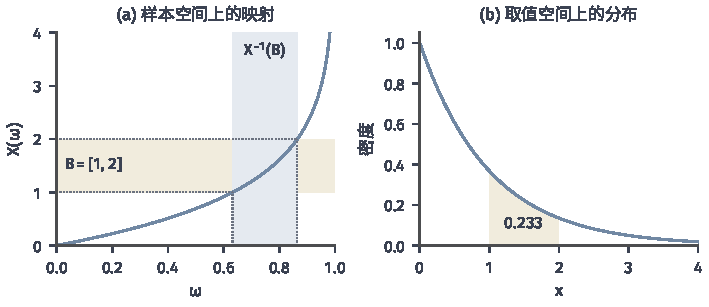
\includegraphics[width=120mm]{figures/02-abstract-mathematics/02-probability-spaces/matplotlib/pmod-pushforward-exponential/figure.pdf}
  \caption{推前测度的两种读法。$[0,1)$均匀模型上$X(\omega)=-\ln(1-\omega)$，$B=[1,2]$。(a) 样本空间上，$B$（黄色横带）的原像是区间$[1-e^{-1},1-e^{-2}]$（蓝色竖带），长度约$0.233$；(b) 取值空间上，$P_X$为指数分布，$B$上的密度面积同为$e^{-1}-e^{-2}\approx0.233$。}
  \label{fig:pmod-pushforward-exponential}
\end{figure*}

\paragraph{概率表、密度与分布函数}
卷一计算分布时用的三种工具，都是$P_X$的不同表示。
离散随机变量的概率表$p(x)=\mathbb P(X=x)$给出$P_X=\sum_xp(x)\delta_x$；有密度$f$的随机变量满足$P_X(B)=\int_Bf(x)\,dx$，这正是说$P_X$相对长度绝对连续，$f$是它的相对密度。
第三种工具是\term{分布函数}（distribution function）$F_X(x)=\mathbb P(X\le x)$，它对任何实值随机变量都存在。

分布函数完全确定分布。
半直线族$\{(-\infty,a]:a\in\mathbb R\}$加上$\mathbb R$本身，对有限交封闭并生成$\mathcal B(\mathbb R)$；两个概率测度若在这些集合上取值相同，由定理~\ref{thm:measure-pi-lambda-uniqueness}，它们在整个$\mathcal B(\mathbb R)$上相同。
所以$F_X=F_Y$当且仅当$P_X=P_Y$。
这解释了卷一的做法：先求分布函数，再求导得到密度，背后识别的始终是同一个测度$P_X$；分布函数在概率表与密度都不存在时仍然可用，例如章首的等待时间和Cantor分布。
这些基本计算的具体做法可参考\BookChapterRef{chap:random-variables}{卷一“随机变量与概率分布”章}。

\paragraph{变换后的分布}
对可测映射$g$，$g(X)$的分布由原像直接确定：
\[
  P_{g(X)}(C)=\mathbb P\bigl(X\in g^{-1}(C)\bigr)=P_X\bigl(g^{-1}(C)\bigr),
  \qquad\text{即}\qquad P_{g(X)}=g_\#P_X.
\]
求变换后的分布时，应先写出事件的原像，再看是否能用密度换元公式化简。
取$X$服从$[0,1]$上的均匀分布，$Y=X^2$。对$0\le y\le1$，
\[
  \mathbb P(Y\le y)=\mathbb P\bigl(X\le\sqrt y\bigr)=\sqrt y,
\]
求导得$Y$在$(0,1)$上的密度$1/(2\sqrt y)$，与第~\ref{sec:measure-cross-space}节的换元公式（取$(0,1)$上的光滑可逆映射$x\mapsto x^2$）一致。
若$g(x)=\mathbb I_{\{x>1/2\}}$，换元公式无从使用，因为$Y=g(X)$只取$0,1$，没有密度；原像方法照样给出$\mathbb P(Y=1)=\mathbb P(X>1/2)=1/2$。

随机对象$X$与它的分布$P_X$是不同类型的对象。
$X$是$\Omega$上的映射，记录每个结果对应哪个取值；$P_X$是$E$上的测度，只记录各取值集合上一共有多少概率。
从$X$可以算出$P_X$，从$P_X$却不能恢复$X$：许多不同的映射会推出同一个测度。
下一小节专门讨论这一差别。

\subsection{同分布与几乎处处相等}

\paragraph{三种相等关系}
说两个随机量“相同”，可以有三种不同强度的含义。

\begin{definition}[同分布]
\label{def:pmod-identical-distribution}
设$X$与$Y$取值于同一个可测空间$(E,\mathcal E)$，它们可以定义在不同的概率空间上。若$P_X=P_Y$，称$X$与$Y$\term{同分布}（identically distributed），记为$X\overset{d}{=}Y$。
\end{definition}

另外两种相等都要求$X,Y$定义在同一个概率空间上。
\emph{处处相等}指$X(\omega)=Y(\omega)$对每个$\omega$成立；\emph{几乎处处相等}（也说几乎必然相等）指它们在某个零概率事件之外相等，记为$X=Y$ a.s.。
对实值或有限维随机向量，$\{X\ne Y\}$本身是事件，几乎处处相等就是$\mathbb P(X\ne Y)=0$。

三者之间有单向的蕴含：处处相等蕴含几乎处处相等，几乎处处相等蕴含同分布。
后一步是因为对每个$B$，$\{X\in B\}$与$\{Y\in B\}$只在$\{X\ne Y\}$上可能不同，
\[
  \bigl|\mathbb P(X\in B)-\mathbb P(Y\in B)\bigr|\le\mathbb P(X\ne Y)=0.
\]
前两种相等比较的是同一个样本点上的取值，所以必须有共同的概率空间；同分布只比较取值空间上的两个测度，可以跨越不同的试验。
例如今天掷的公平硬币与明天掷的公平硬币同分布，但问“两枚硬币是否几乎处处相等”，要先把两次试验放进同一个概率空间才有意义。

\paragraph{同分布而不相等}
同分布推不出几乎处处相等，最简单的例子来自一次翻转。

\begin{example}[均匀变量与它的翻转]
\label{ex:pmod-reflection-uniform}
在$[0,1]$均匀模型上令$X(\omega)=\omega$，$Y(\omega)=1-\omega$。
对$0\le x\le1$，$\mathbb P(Y\le x)=\mathbb P(\omega\ge1-x)=x=\mathbb P(X\le x)$，所以$X\overset{d}{=}Y$，两者都服从$[0,1]$上的均匀分布。
但$X(\omega)=Y(\omega)$只在$\omega=1/2$时成立，$\mathbb P(X=Y)=0$；平均距离$\mathbb E|X-Y|=\int_0^1|2\omega-1|\,d\omega=1/2$。
\end{example}

图~\ref{fig:pmod-reflection-uniform}左图在样本空间上比较两者：对同一个$\omega$，两条直线给出不同的值，竖线标出$\omega=1/4$处的差距$1/2$。
右图在取值空间上比较两者：两条分布函数完全重合。
分布只看右图，所以无法区分$X$与$Y$；任何只依赖分布的量，例如$\mathbb P(X>0.9)$或$\mathbb E X^2$，两者都相同。

\begin{figure}[htbp]
  \centering
  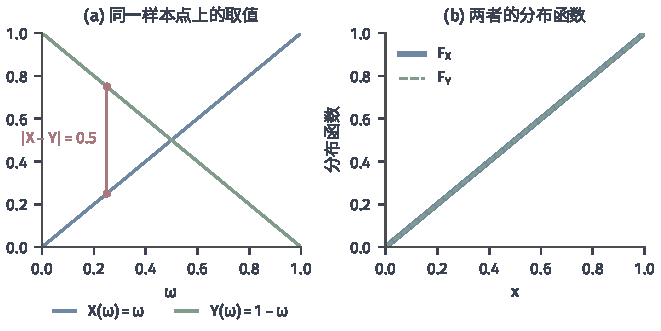
\includegraphics[width=112mm]{figures/02-abstract-mathematics/02-probability-spaces/matplotlib/pmod-reflection-uniform/figure.pdf}
  \caption{$[0,1]$均匀模型上的$X(\omega)=\omega$与$Y(\omega)=1-\omega$。(a) 同一样本点上的取值，竖线标出$\omega=1/4$处$|X-Y|=1/2$，两者只在$\omega=1/2$处相等；(b) 两者的分布函数都是$F(x)=x$，图中完全重合。}
  \label{fig:pmod-reflection-uniform}
\end{figure}

\paragraph{相同边缘下的不同轨迹}
同样的现象出现在随机变量列中，而且影响更大：各项的分布相同，不能决定整列在样本点上的行为。

\begin{example}[常值比特列与交替比特列]
\label{ex:pmod-alternating-bits}
设$Z\sim\operatorname{Bernoulli}(1/2)$，例如在$[0,1)$均匀模型上取$Z=\mathbb I_{\{\omega\ge1/2\}}$。
令$X_n=Z$对一切$n$成立，并令
\[
  Y_n=\begin{cases}Z,&n\text{为奇数},\\1-Z,&n\text{为偶数}.\end{cases}
\]
由于$1-Z$也服从$\operatorname{Bernoulli}(1/2)$，每个$X_n$与每个$Y_n$都服从$\operatorname{Bernoulli}(1/2)$，两列的各项分布完全相同。
但$X_n(\omega)$对每个$\omega$都是常数列，处处收敛；$Y_n(\omega)$对每个$\omega$都在$0$与$1$之间交替，处处不收敛。
两列的差别在多项之间的联合规律上：$\mathbb P(X_1=X_2)=1$，而$\mathbb P(Y_1=Y_2)=0$。
\end{example}

图~\ref{fig:pmod-alternating-paths}分别画出$Z=0$与$Z=1$时两列的取值。
圆点构成的$X_n$是水平线；方块构成的$Y_n$锯齿式跳动，对两种$Z$都是如此。
如果只记录“第$n$项服从什么分布”，这两张图给不出任何区别。
因此第~\ref{chap:random-variable-convergence}章研究随机变量列在同一样本点上的收敛时，必须使用共同的概率空间；而第~\ref{chap:weak-convergence-limit-theorems}章只比较分布时，这两列都平凡地“分布收敛”到$\operatorname{Bernoulli}(1/2)$，样本点上的差别被完全忽略。

\begin{figure}[htbp]
  \centering
  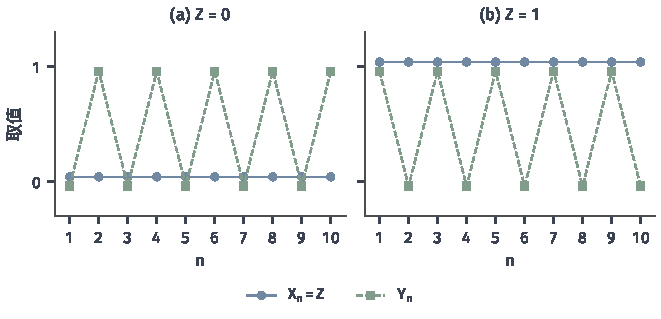
\includegraphics[width=112mm]{figures/02-abstract-mathematics/02-probability-spaces/matplotlib/pmod-alternating-paths/figure.pdf}
  \caption{同一公平比特$Z$构造的两列随机变量，横轴为下标$n=1,\dots,10$。圆点为$X_n=Z$，方块为在$Z$与$1-Z$之间交替的$Y_n$。(a) $Z=0$；(b) $Z=1$。为避免重合，两列在竖直方向各错开$0.04$。两列每一项都服从$\operatorname{Bernoulli}(1/2)$，但前者处处收敛，后者处处不收敛。}
  \label{fig:pmod-alternating-paths}
\end{figure}

\subsection{联合分布与边缘分布}

\paragraph{联合分布的定义}
例~\ref{ex:pmod-alternating-bits}说明，比较多个随机对象时需要它们一起出现的规律。
上一节已经把有限个随机对象合成为乘积空间中的一个可测映射，它的分布就是这种规律。

\begin{definition}[联合分布与边缘分布]
\label{def:pmod-joint-distribution}
设$X_1,\dots,X_m$定义在同一个概率空间上，$X_i$取值于$(E_i,\mathcal E_i)$。
随机对象$(X_1,\dots,X_m)$在$(E_1\times\cdots\times E_m,\ \mathcal E_1\otimes\cdots\otimes\mathcal E_m)$上的分布
\[
  P_{(X_1,\dots,X_m)}(C)=\mathbb P\bigl((X_1,\dots,X_m)\in C\bigr)
\]
称为$X_1,\dots,X_m$的\term{联合分布}（joint distribution）；相对于它，每个$P_{X_i}$称为\term{边缘分布}（marginal distribution）。
\end{definition}

边缘分布由联合分布唯一确定。
记坐标投影$\pi_i(x_1,\dots,x_m)=x_i$，则$X_i=\pi_i\circ(X_1,\dots,X_m)$，由推前的复合规则，
\[
  P_{X_i}=(\pi_i)_\#P_{(X_1,\dots,X_m)},\qquad
  P_{X_i}(B)=P_{(X_1,\dots,X_m)}\bigl(E_1\times\cdots\times B\times\cdots\times E_m\bigr).
\]
在概率表中，这就是按行或按列求和；在密度模型中，这就是对其余坐标积分。
这里不要求联合分布有密度，也不要求$E_i$是实轴：定义只用到乘积可测结构与推前。

\paragraph{边缘不能决定联合}
反过来，各个边缘一般不能恢复联合分布。
具有给定边缘的联合分布称为这些边缘的一个\term{耦合}（coupling）；同一组边缘通常有许多耦合。

\begin{example}[相同边缘的三种配对]
\label{ex:pmod-bernoulli-couplings}
在$[0,1)$均匀模型上令$X=\mathbb I_{\{\omega\ge1/2\}}$，并考虑三种$Y$：
\[
  Y^{(a)}=X,\qquad Y^{(b)}=1-X,\qquad
  Y^{(c)}=\mathbb I_{\{\omega\in[1/4,1/2)\cup[3/4,1)\}}.
\]
三个$Y$都服从$\operatorname{Bernoulli}(1/2)$，与$X$的边缘也相同。
三种联合概率表依次为：同向配对把概率$1/2,1/2$放在对角格$(0,0),(1,1)$上；反向配对放在反对角格$(0,1),(1,0)$上；第三种配对中，例如$\mathbb P(X=1,Y^{(c)}=1)=\mathbb P([3/4,1))=1/4$，四格都是$1/4$。
于是$\mathbb P(X=Y)$依次为$1,0,1/2$，$\mathbb P(X+Y=2)$依次为$1/2,0,1/4$，协方差依次为$1/4,-1/4,0$。
\end{example}

图~\ref{fig:pmod-bernoulli-couplings}列出了三张表。
三张表的行和、列和完全相同，都是$(1/2,1/2)$，差别只在四个格子之间如何分配概率。
所以边缘分布缺少的不是某个单独对象的参数，而是“哪些取值同时出现”的规律；任何同时涉及$X$与$Y$的量，例如$X+Y$的分布、$\mathbb P(X=Y)$或协方差，都要由联合分布决定。
第三种配对的四格恰好等于边缘之积，下一节会看到这正是独立的情形。
在给定边缘的众多耦合中如何比较与挑选，属于卷四“概率分布”部分的问题。

\begin{figure*}[htbp]
  \centering
  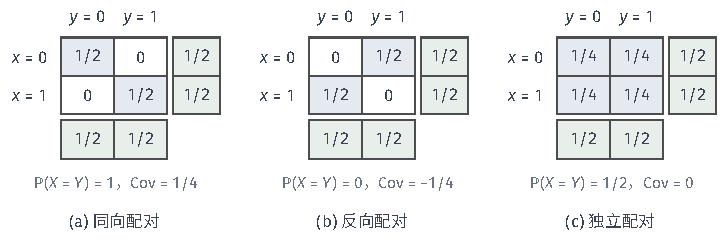
\includegraphics[width=122mm]{figures/02-abstract-mathematics/02-probability-spaces/tikz/pmod-bernoulli-couplings/figure.pdf}
  \caption{两个$\operatorname{Bernoulli}(1/2)$变量的三种联合概率表。行为$X$的取值，列为$Y$的取值，绿色格为边缘概率，蓝色格为取正概率的组合。(a) 同向配对$Y=X$；(b) 反向配对$Y=1-X$；(c) 独立配对，四格都等于边缘之积。三表的边缘完全相同，$\mathbb P(X=Y)$与协方差却不同。}
  \label{fig:pmod-bernoulli-couplings}
\end{figure*}

\section{独立性}
\label{sec:pmod-independence}

联合分布写清了多个观测一起出现的规律。
在例~\ref{ex:pmod-bernoulli-couplings}的三种配对中，只有第三种的联合概率表恰好等于边缘之积：知道$X$的取值，对$Y$落在哪里没有任何影响。
本节把这种“没有概率依赖”的关系推广到一般随机对象，证明它等价于联合分布分解为乘积测度，并说明它在变换与分组之后如何保留。

\subsection{事件族与随机对象的独立性}

\paragraph{从事件的乘法判据到$\sigma$代数}
卷一称事件$A_1,\dots,A_n$相互独立，是指其中任意一部分事件之交的概率等于各自概率之积。
这个条件也自动覆盖了补事件：例如由$\mathbb P(A\cap B)=\mathbb P(A)\mathbb P(B)$可得
\[
  \mathbb P\bigl((\Omega\setminus A)\cap B\bigr)=\mathbb P(B)-\mathbb P(A\cap B)=\mathbb P(\Omega\setminus A)\,\mathbb P(B).
\]
所以一个事件$A$的独立性，实际上是它生成的整个$\sigma$代数$\{\varnothing,A,\Omega\setminus A,\Omega\}$的独立性。
对随机对象，我们关心的是它能判断的全部事件，即$\sigma(X)$；这提示我们直接对$\sigma$代数定义独立。

\begin{definition}[$\sigma$代数与随机对象的独立性]
\label{def:pmod-independence}
设$(\Omega,\mathcal F,\mathbb P)$是概率空间，$(\mathcal G_i)_{i\in I}$是一族子$\sigma$代数，$\mathcal G_i\subseteq\mathcal F$，指标集$I$可以有限、可数或更大。
若对每个有限非空子集$J\subseteq I$及任意选取的$A_j\in\mathcal G_j$（$j\in J$），都有
\[
  \mathbb P\Bigl(\bigcap_{j\in J}A_j\Bigr)=\prod_{j\in J}\mathbb P(A_j),
\]
就称这族$\sigma$代数\term{相互独立}（independent）。
一族随机对象$(X_i)_{i\in I}$称为相互独立，若$(\sigma(X_i))_{i\in I}$相互独立；随机对象$X$与$Y$独立记为$X\perp Y$。
\end{definition}

按$\sigma(X_i)$的定义，随机对象的独立就是：对每个有限的$J$和任意可测集$B_j$，
$\mathbb P(X_j\in B_j,\ j\in J)=\prod_{j\in J}\mathbb P(X_j\in B_j)$。
事件$A_i$的独立等价于示性变量$\mathbb I_{A_i}$的独立，也等价于$\sigma$代数$\{\varnothing,A_i,\Omega\setminus A_i,\Omega\}$的独立。
于是事件独立、变量独立与信息独立都落在同一个乘法判据上。

\paragraph{随机族的相互独立}
定义只对有限子族提出要求，并不会漏掉可数交：若$A_k\in\mathcal G_{i_k}$，指标$i_k$互不相同，则有限交$\bigcap_{k\le n}A_k$随$n$单调减少，由概率的连续性，
\[
  \mathbb P\Bigl(\bigcap_{k=1}^\infty A_k\Bigr)=\lim_{n\to\infty}\prod_{k=1}^n\mathbb P(A_k)=\prod_{k=1}^\infty\mathbb P(A_k).
\]
所以可数交的乘法公式由有限子族的乘法公式自动推出，不必另加要求。
另一方面，定义要求\emph{所有}有限子族满足乘法公式，而不仅仅是每一对。

\begin{example}[两个比特及其模二和]
\label{ex:pmod-xor-bits}
设$X,Y$是独立的公平比特，$Z=X\oplus Y$为它们的模二和：$X=Y$时$Z=0$，否则$Z=1$。
样本空间可取$\Omega=\{00,01,10,11\}$，每点概率$1/4$。
任取两个变量，它们的四种取值组合各占一个样本点，所以每对都独立，即三者\term{两两独立}（pairwise independent）；但
\[
  \mathbb P(X=1,Y=1,Z=1)=0\ne\frac18=\mathbb P(X=1)\mathbb P(Y=1)\mathbb P(Z=1),
\]
三者不相互独立。
\end{example}

卷一用概率表验证过这个例子，这里补充它在信息层面的原因。
图~\ref{fig:pmod-xor-partitions}把$\sigma(X)$、$\sigma(Y)$、$\sigma(Z)$画成同一个$2\times2$网格的三种二分：竖切、横切与对角配色。
任意两种二分叠加，都把网格切成四个各占$1/4$的格子，这就是两两独立。
但$Z$是$(X,Y)$的函数，由式~\eqref{eq:pmod-function-information}，$\sigma(Z)\subseteq\sigma(X,Y)$：图中第四个网格的每一格内$Z$都已确定。
一个事件$A$若与自身独立，则$\mathbb P(A)=\mathbb P(A)^2$，只能取$0$或$1$；因此$\{Z=1\}$这个概率为$1/2$的事件不可能独立于包含它的$\sigma(X,Y)$。
本节稍后的定理~\ref{thm:pmod-independence-grouping}将说明，三者若相互独立，$\sigma(Z)$就必须与$\sigma(X,Y)$独立；这正是相互独立失败的信息层面原因。
两两检查看不到这一点，因为它只比较单个变量的信息，从不把$X$与$Y$的信息合起来。

\begin{figure}[htbp]
  \centering
  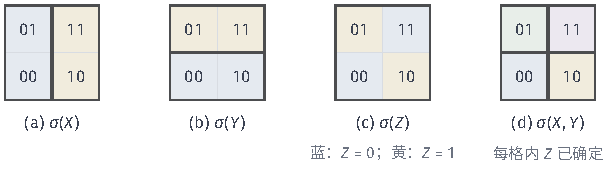
\includegraphics[width=104mm]{figures/02-abstract-mathematics/02-probability-spaces/tikz/pmod-xor-partitions/figure.pdf}
  \caption{两个独立公平比特$X,Y$与$Z=X\oplus Y$生成的信息。四格分别表示样本点$xy$，各有概率$1/4$，第一位$x$为列、第二位$y$为行。(a)(b)(c) 依次为$\sigma(X)$、$\sigma(Y)$、$\sigma(Z)$的两个块（同色为一块，(c)中蓝色为$Z=0$，黄色为$Z=1$）；任两种划分交出四个各$1/4$的格子。(d) $\sigma(X,Y)$把四格全部分开，每格中$Z$已经确定，所以$Z$不能独立于$(X,Y)$。}
  \label{fig:pmod-xor-partitions}
\end{figure}

\subsection{联合分布的乘积分解}

\paragraph{生成族上的独立性判据}
按定义验证独立，要对$\sigma(X_i)$中的全部事件检查乘法公式，这通常做不到。
与测度唯一性一样，我们希望只在一个生成族上检查。

\begin{lemma}[生成族上的独立性判据]
\label{lem:pmod-pi-independence}
设$\mathcal G_1,\dots,\mathcal G_n$是$\mathcal F$的子$\sigma$代数，$\mathcal C_i$是对有限交封闭的集合族，$\Omega\in\mathcal C_i$，且$\sigma(\mathcal C_i)=\mathcal G_i$。
若对任意$C_i\in\mathcal C_i$（$i=1,\dots,n$）都有
$\mathbb P(C_1\cap\cdots\cap C_n)=\prod_{i=1}^n\mathbb P(C_i)$，
则$\mathcal G_1,\dots,\mathcal G_n$相互独立。
\end{lemma}

\begin{proof}
固定$C_2\in\mathcal C_2,\dots,C_n\in\mathcal C_n$，在$\mathcal G_1$上比较两个有限测度
\[
  \mu(A)=\mathbb P(A\cap C_2\cap\cdots\cap C_n),\qquad
  \nu(A)=\mathbb P(A)\prod_{i=2}^n\mathbb P(C_i).
\]
由假设，$\mu$与$\nu$在$\mathcal C_1$上相等；$\mathcal C_1$包含$\Omega$，对有限交封闭且生成$\mathcal G_1$，由定理~\ref{thm:measure-pi-lambda-uniqueness}，$\mu=\nu$在整个$\mathcal G_1$上成立。
于是乘法公式在$\mathcal C_1$换成$\mathcal G_1$后仍然成立。
对第二个坐标重复同样的论证（此时第一个坐标已可任取$\mathcal G_1$中的事件），依次进行$n$步，得到乘法公式对任意$A_i\in\mathcal G_i$成立。
最后，对子集$J\subseteq\{1,\dots,n\}$，在$i\notin J$处取$A_i=\Omega$，即得定义要求的每个有限子族的乘法公式。
\end{proof}

对无穷族$(\mathcal G_i)_{i\in I}$，只需对每个有限子族应用引理。

\paragraph{独立与乘积测度}
现在可以把独立性完全翻译成联合分布的性质。
概率测度是有限测度，第~\ref{sec:measure-general-structure}节保证有限个概率测度的乘积测度在乘积$\sigma$代数上存在且唯一，它由矩形上的取值$\prod_iP_i(B_i)$决定。

\begin{theorem}[独立与乘积分解]
\label{thm:pmod-independence-product}
设$X_1,\dots,X_n$定义在同一个概率空间上，$X_i$取值于$(E_i,\mathcal E_i)$。
则$X_1,\dots,X_n$相互独立，当且仅当在$\mathcal E_1\otimes\cdots\otimes\mathcal E_n$上
\[
  P_{(X_1,\dots,X_n)}=P_{X_1}\otimes\cdots\otimes P_{X_n}.
\]
\end{theorem}

\begin{proof}
可测矩形$R=B_1\times\cdots\times B_n$（$B_i\in\mathcal E_i$）构成的族对有限交封闭，包含整个乘积空间，并生成乘积$\sigma$代数。
在矩形上，
\[
  \begin{aligned}
  P_{(X_1,\dots,X_n)}(R)&=\mathbb P\Bigl(\bigcap_{i=1}^n\{X_i\in B_i\}\Bigr),\\
  (P_{X_1}\otimes\cdots\otimes P_{X_n})(R)&=\prod_{i=1}^n\mathbb P(X_i\in B_i).
  \end{aligned}
\]
若$X_1,\dots,X_n$独立，两式右侧相等，于是两个概率测度在矩形上相等；由定理~\ref{thm:measure-pi-lambda-uniqueness}，它们在整个乘积$\sigma$代数上相等。
反之，若两个测度相等，把它们作用于矩形即得$\mathbb P(\bigcap_i\{X_i\in B_i\})=\prod_i\mathbb P(X_i\in B_i)$对一切$B_i$成立；取部分$B_i=E_i$就得到每个子族的乘法公式。
\end{proof}

证明的关键在唯一性那一步。
独立性的定义只直接给出矩形事件的概率；乘积空间中的大多数事件，例如$\{X<Y\}$或$\{X^2+Y^2\le1\}$，都不是矩形。
定理说明，一旦矩形上的乘法公式成立，这些事件的概率也随之由乘积测度确定，可以用累次积分计算。

\begin{example}[两个独立均匀变量的比较]
\label{ex:pmod-independent-uniform-order}
设$X,Y$独立，都服从$[0,1)$上的均匀分布。
由定理~\ref{thm:pmod-independence-product}，$(X,Y)$的联合分布是单位正方形上的面积。
矩形事件$\{X\in[0.2,0.6),\,Y\in[0.5,0.9)\}$的概率是$0.4\times0.4=0.16$。
非矩形事件$\{X<Y\}$的概率要对乘积测度积分；按$x$切片，第~\ref{sec:measure-general-structure}节的Tonelli定理给出
\[
  \mathbb P(X<Y)=\int_0^1\mathbb P(Y>x)\,dx=\int_0^1(1-x)\,dx=\frac12.
\]
\end{example}

图~\ref{fig:pmod-product-rectangle}对照了两种事件。
左图的矩形面积等于两条边长之积，这正是独立性在矩形上的直接含义；右图的三角形不是矩形，它的面积来自乘积测度的唯一扩张，再按竖直切片累加。

\begin{figure}[htbp]
  \centering
  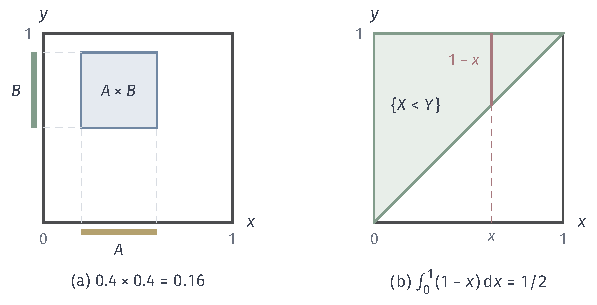
\includegraphics[width=100mm]{figures/02-abstract-mathematics/02-probability-spaces/tikz/pmod-product-rectangle/figure.pdf}
  \caption{$X,Y$独立且都服从$[0,1)$上的均匀分布时，联合分布为单位正方形上的面积。(a) 矩形$A\times B$，$A=[0.2,0.6)$，$B=[0.5,0.9)$，概率为边缘概率之积$0.16$；(b) 非矩形事件$\{X<Y\}$，在横坐标$x$处的切片长度为$1-x$，按切片积分得$1/2$。}
  \label{fig:pmod-product-rectangle}
\end{figure}

\paragraph{分布函数与密度判据}
对实值随机变量，生成族还可以进一步缩小。
半直线的原像$\{X_i\le a\}$（$a\in\mathbb R$）连同$\Omega$构成对有限交封闭的族；由于满足$X_i^{-1}(B)\in\sigma(\{X_i\le a\}:a\in\mathbb R)$的$B$构成包含全部半直线的$\sigma$代数，这一族生成$\sigma(X_i)$。
由引理~\ref{lem:pmod-pi-independence}，实值随机变量$X_1,\dots,X_n$相互独立，当且仅当
\begin{equation}
  \mathbb P(X_1\le a_1,\dots,X_n\le a_n)=\prod_{i=1}^n\mathbb P(X_i\le a_i)\qquad\text{对一切}\ a_1,\dots,a_n\in\mathbb R.
  \label{eq:pmod-cdf-factorization}
\end{equation}
（取部分$a_i\to+\infty$即得到含$\Omega$的情形。）
由分布函数的右连续性，只需对有理数$a_i$核对，再取有理数从右侧逼近即可。

若$(X,Y)$有联合密度$f$，独立等价于
\[
  f(x,y)=f_X(x)f_Y(y)\qquad\text{对几乎每个}\ (x,y)\in\mathbb R^2,
\]
其中$f_X,f_Y$是边缘密度。
若乘积式成立，Tonelli定理给出$\mathbb P(X\in A,Y\in B)=\int_Af_X\,dx\int_Bf_Y\,dy$，即独立；
反之，独立时联合分布等于$P_X\otimes P_Y$，后者在矩形上（从而由唯一性在全部Borel集上）以$f_X(x)f_Y(y)$为密度，同一测度的两个密度几乎处处相等（定理~\ref{thm:measure-radon-nikodym}）。
“几乎每个”不能去掉：在一条线段上改动$f$不改变任何概率。

乘积分解是独立的\emph{条件}，不是联合分布的一般形式。
例~\ref{ex:pmod-bernoulli-couplings}的同向与反向配对都有完全确定的联合分布，却不能写成边缘之积。

\subsection{独立性的保持与分组}

\paragraph{变换与分组}
实际中常把独立的观测分组汇总：先算前一半样本的均值，再算后一半样本的最大值。
我们希望知道，各组的汇总结果是否仍然独立。

\begin{theorem}[分组与变换保持独立]
\label{thm:pmod-independence-grouping}
设$(\mathcal G_i)_{i\in I}$是相互独立的子$\sigma$代数族，$I$被分成互不相交的子集$I_k$（$k\in K$）。令
$\mathcal H_k=\sigma\bigl(\bigcup_{i\in I_k}\mathcal G_i\bigr)$，则$(\mathcal H_k)_{k\in K}$相互独立。
特别地，若随机对象$(X_i)_{i\in I}$相互独立，各$I_k$有限，$f_k$是定义在$(X_i)_{i\in I_k}$取值空间上的可测函数，则$Y_k=f_k\bigl((X_i)_{i\in I_k}\bigr)$（$k\in K$）相互独立。
\end{theorem}

\begin{proof}
对每个$k$，令$\mathcal C_k$为形如$A_{i_1}\cap\cdots\cap A_{i_r}$的集合全体，其中$i_1,\dots,i_r$是$I_k$中有限个互不相同的指标，$A_{i_l}\in\mathcal G_{i_l}$；约定空交为$\Omega$。
两个这样的集合相交时，同一指标的事件在$\mathcal G_i$内相交，结果仍属于$\mathcal C_k$，所以$\mathcal C_k$对有限交封闭；它包含每个$\mathcal G_i$（$i\in I_k$），并含于$\mathcal H_k$，因此生成$\mathcal H_k$。

取有限个不同的$k_1,\dots,k_m$及$C_l\in\mathcal C_{k_l}$。
各$C_l$用到的指标属于不相交的$I_{k_l}$，所以$C_1\cap\cdots\cap C_m$是有限个来自不同$\mathcal G_i$的事件之交；由独立性，其概率等于所有这些事件概率之积。
把乘积按组归并，每组的乘积再由独立性等于$\mathbb P(C_l)$，于是
$\mathbb P(C_1\cap\cdots\cap C_m)=\prod_{l=1}^m\mathbb P(C_l)$。
由引理~\ref{lem:pmod-pi-independence}，$\mathcal H_{k_1},\dots,\mathcal H_{k_m}$相互独立；由于$k_1,\dots,k_m$是任取的有限个指标，整族$(\mathcal H_k)$相互独立。

对第二个结论，取$\mathcal G_i=\sigma(X_i)$。
$\sigma\bigl((X_i)_{i\in I_k}\bigr)$是包含各$\sigma(X_i)$的最小$\sigma$代数，即$\mathcal H_k$；由式~\eqref{eq:pmod-function-information}，$\sigma(Y_k)\subseteq\mathcal H_k$。
独立的$\sigma$代数的子$\sigma$代数仍满足乘法公式，所以$Y_k$相互独立。
\end{proof}

定理的第一个结论对组数和组的大小都没有有限性要求：可数多组、每组可数多个变量时，有限交组成的生成族和测度唯一性把乘法公式从有限个事件延伸到整个$\mathcal H_k$。
第二个结论要求各组有限，只是为了让$(X_i)_{i\in I_k}$取值于有限乘积空间；组内变量无穷时，任何$\mathcal H_k$可测的随机变量仍由第一个结论得到独立性。
例如$X_1,\dots,X_4$相互独立时，$X_1+X_2$与$X_3X_4$独立，$\max\{X_1,X_2\}$与$X_3$独立。
例~\ref{ex:pmod-xor-bits}正是从反面使用这个定理：把$\{X,Y\}$与$\{Z\}$分成两组，相互独立会迫使$\sigma(Z)$与$\sigma(X,Y)$独立，而概率为$1/2$的事件$\{Z=1\}$同属两者，这已经排除。

\paragraph{独立同分布族}
一族随机变量称为\term{独立同分布}（independent and identically distributed，i.i.d.），若它们相互独立并且服从同一个分布。
两个要求各管一件事：同分布只约束每个变量的边缘，独立约束它们的联合分布必须是边缘的乘积。
例~\ref{ex:pmod-alternating-bits}中的$Y_n$满足前者而不满足后者。

一个概率空间上能否容纳无穷多个独立的随机变量？$[0,1)$均匀模型就可以。

\begin{example}[二进制数字是独立的公平比特]
\label{ex:pmod-binary-digits}
对$\omega\in[0,1)$，令$d_k(\omega)=\lfloor2^k\omega\rfloor\bmod2$为它二进制展开（取不以无穷个$1$结尾的展开）的第$k$位。
对任意$n$及$b_1,\dots,b_n\in\{0,1\}$，事件$\{d_1=b_1,\dots,d_n=b_n\}$是一个长$2^{-n}$的二进区间，所以其概率为$2^{-n}$。
对$b_1,\dots,b_{n-1}$求和得$\mathbb P(d_n=b_n)=1/2$，于是
$\mathbb P(d_1=b_1,\dots,d_n=b_n)=\prod_{k=1}^n\mathbb P(d_k=b_k)$。
每个$\sigma(d_k)$只含$\varnothing,\{d_k=0\},\{d_k=1\},\Omega$四个事件，乘法公式在含$\Omega$的选取下由对相应$b_k$求和得到；由引理~\ref{lem:pmod-pi-independence}，$(d_k)_{k\ge1}$是独立同分布的$\operatorname{Bernoulli}(1/2)$序列。
\end{example}

例~\ref{ex:pmod-bernoulli-couplings}中的$X$与$Y^{(c)}$正是$d_1$与$d_2$，所以第三种配对是独立配对。
用这列数字还能造出更多对象：$\sum_k2d_k3^{-k}$服从第~\ref{sec:pmod-probability-space}节的Cantor分布；把数字分成无穷多组不相交的无穷子列，第$j$组的数字$d_{k_{j,1}},d_{k_{j,2}},\dots$重新排成$U_j=\sum_l d_{k_{j,l}}2^{-l}$，它与$\omega$本身同分布，即服从$[0,1)$上的均匀分布；$U_j$关于第$j$组生成的$\sigma$代数可测，由定理~\ref{thm:pmod-independence-grouping}的第一个结论，$U_1,U_2,\dots$相互独立。
本章研究的都是已经定义在给定概率空间上的随机族；由一套相容的有限维分布构造整个随机过程，以及一般指标集上的扩张定理，放在卷三“过程与轨迹演化”部分。

\section{期望与积分}
\label{sec:pmod-expectation}

卷一的期望有两种算法：离散时对概率表加权求和，有密度时对密度积分。
章首的等待时间两者都不适用。
本节把期望定义为对概率测度的积分，于是两种算法成为同一个定义的两种特例；再讨论矩条件控制了什么，以及几个后续章节反复使用的不等式。

\subsection{一般期望与分布积分}

\paragraph{期望的定义}
第~\ref{sec:measure-general-structure}节已经对一般测度定义了积分：非负函数的积分由简单函数从下逼近，可以取$+\infty$；有符号函数拆成正负两部分分别积分。
把它用于概率测度，就得到期望。

\begin{definition}[期望]
\label{def:pmod-expectation}
设$X$是概率空间$(\Omega,\mathcal F,\mathbb P)$上的随机变量。
若$X\ge0$，定义$\mathbb E X=\int_\Omega X\,d\mathbb P\in[0,+\infty]$。
一般情形记$X^+=\max\{X,0\}$，$X^-=\max\{-X,0\}$；当$\mathbb EX^+$与$\mathbb EX^-$不同时为$+\infty$时，定义$\mathbb EX=\mathbb EX^+-\mathbb EX^-$，称为$X$的\term{期望}（expectation）。
若$\mathbb E|X|<\infty$，称$X$\term{可积}（integrable）。
复值随机变量$X=U+\mathrm iV$在$\mathbb E|X|<\infty$时定义$\mathbb EX=\mathbb EU+\mathrm i\,\mathbb EV$。
\end{definition}

定义中的限制是为了排除$\infty-\infty$。
例如Cauchy分布的变量满足$\mathbb EX^+=\mathbb EX^-=+\infty$，它的期望没有定义；而一个非负变量的期望可以是$+\infty$，这时它是有定义的，只是不有限。
可积变量的期望具有线性与单调性，并且$|\mathbb EX|\le\mathbb E|X|$；对事件$A$，$\mathbb E\,\mathbb I_A=\mathbb P(A)$。
几乎必然相等的两个随机变量期望相同，因为积分不受零概率集合上取值的影响。

\paragraph{在取值空间上计算期望}
定义中的积分是在样本空间上进行的，可是实际计算时我们几乎从不知道$\Omega$的样子，只知道$X$的分布。
推前测度的积分公式把计算搬到取值空间。

\begin{theorem}[分布积分公式]
\label{thm:pmod-change-of-variables}
设$X$是取值于$(E,\mathcal E)$的随机对象，$g:E\to[0,+\infty]$可测，则
\[
  \mathbb E\,g(X)=\int_Eg\,dP_X.
\]
对可测的$g:E\to\mathbb R$，$g(X)$可积当且仅当$\int_E|g|\,dP_X<\infty$，此时上式仍成立。
\end{theorem}

\begin{proof}
这是式~\eqref{eq:measure-pushforward-integral}取$T=X$、$\mu=\mathbb P$的情形。
其机制是：$g=\mathbb I_B$时两边都等于$\mathbb P(X\in B)=P_X(B)$；由线性，等式对非负简单函数成立；用非负简单函数单调上升逼近$g$，两边同时应用单调收敛定理，得到非负情形。
有符号情形对$|g|$使用非负情形判断可积，再对$g^+$与$g^-$分别使用非负情形后相减。
\end{proof}

这个公式有两个直接推论。
第一，$\mathbb E\,g(X)$只依赖$P_X$：同分布的随机对象对一切非负或可积的$g$有相同期望，例~\ref{ex:pmod-reflection-uniform}中$\mathbb EX^2=\mathbb EY^2=1/3$。
第二，卷一的两种算法都是它的特例：$P_X=\sum_xp(x)\delta_x$时，由点质量混合的积分得$\mathbb Eg(X)=\sum_xg(x)p(x)$；$P_X$以$f$为密度时，$\int g\,dP_X=\int g(x)f(x)\,dx$，先对示性函数成立，再经简单函数与单调收敛推广。
对多个随机对象，把$g$取为乘积空间上的函数并用联合分布，就得到$\mathbb E\,g(X,Y)=\int g\,dP_{(X,Y)}$。

\paragraph{点质量与连续质量同时存在}
分布积分公式不要求$P_X$有任何特殊表示，因而可以直接处理混合分布。

\begin{example}[有空闲窗口的等待时间]
\label{ex:pmod-mixed-waiting}
设等待时间$X$以概率$0.4$等于$0$，以概率$0.6$服从率参数为$1$的指数分布，即
\[
  P_X=0.4\,\delta_0+0.6\,\mathrm{Exp}(1).
\]
它的分布函数在$x\ge0$时为$F_X(x)=0.4+0.6(1-e^{-x})$，在$0$处跳跃$0.4$。
积分对测度的混合是线性的，所以对非负可测$g$，
\[
  \mathbb E\,g(X)=0.4\,g(0)+0.6\int_0^\infty g(x)e^{-x}\,dx.
\]
取$g(x)=e^{-x}$，得$\mathbb Ee^{-X}=0.4+0.6\times\tfrac12=0.7$。
取$g(x)=x$与$x^2$，得$\mathbb EX=0.6$，$\mathbb EX^2=0.6\times2=1.2$，$\operatorname{Var}X=1.2-0.36=0.84$。
\end{example}

如果把$0.6e^{-x}$误当作$X$的密度，算出的$\mathbb Ee^{-X}$只有$0.3$，而且这个“密度”的总积分只有$0.6$。
图~\ref{fig:pmod-mixed-expectation}显示了遗漏的部分：左图的分布函数在原点有高$0.4$的跳跃，它就是点质量；右图中绿色面积$0.3$来自连续部分，红色竖线代表点质量贡献的$0.4\times g(0)=0.4$。
对$g(x)=x$，点质量的贡献是$0.4\times0=0$，所以只按连续部分算均值碰巧不出错；一旦$g(0)\ne0$，遗漏就会显现。

\begin{figure*}[htbp]
  \centering
  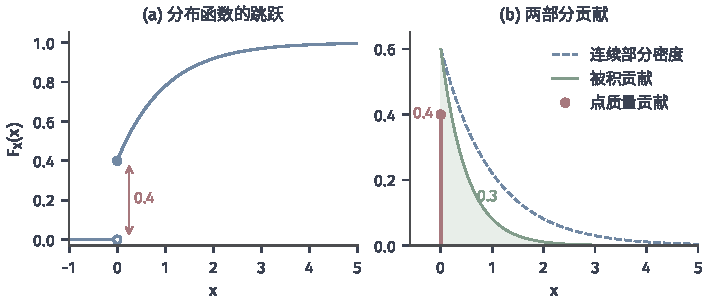
\includegraphics[width=120mm]{figures/02-abstract-mathematics/02-probability-spaces/matplotlib/pmod-mixed-expectation/figure.pdf}
  \caption{混合分布$P_X=0.4\delta_0+0.6\,\mathrm{Exp}(1)$的期望计算。(a) 分布函数在$x=0$处跳跃$0.4$，空心点为左极限；(b) 计算$\mathbb Ee^{-X}$时，虚线为连续部分的密度$0.6e^{-x}$，绿色区域为被积函数$0.6e^{-2x}$，面积$0.3$；红色竖线为点质量的贡献$0.4$。两部分之和为$0.7$。}
  \label{fig:pmod-mixed-expectation}
\end{figure*}

\paragraph{独立对象的乘积期望}
独立性使联合分布成为乘积测度，而乘积测度上的积分可以按坐标分别进行。

\begin{theorem}[独立对象的乘积期望]
\label{thm:pmod-product-expectation}
设$X$与$Y$独立，分别取值于$(E_1,\mathcal E_1)$与$(E_2,\mathcal E_2)$，$g:E_1\to\mathbb R$与$h:E_2\to\mathbb R$可测。
\begin{enumerate}
  \item 若$g,h\ge0$，则$\mathbb E[g(X)h(Y)]=\mathbb Eg(X)\,\mathbb Eh(Y)$，两边在$[0,+\infty]$中取值，约定$0\cdot\infty=0$。
  \item 若$g(X)$与$h(Y)$都可积，则$g(X)h(Y)$可积，且同一等式成立。
\end{enumerate}
特别地，独立可积实值随机变量满足$\mathbb E[XY]=\mathbb EX\,\mathbb EY$。
\end{theorem}

\begin{proof}
由定理~\ref{thm:pmod-change-of-variables}与定理~\ref{thm:pmod-independence-product}，
\[
  \mathbb E[g(X)h(Y)]=\int_{E_1\times E_2}g(x)h(y)\,d(P_X\otimes P_Y)(x,y).
\]
当$g,h\ge0$时，被积函数非负且乘积可测，第~\ref{sec:measure-general-structure}节的Tonelli定理允许先对$y$积分：内层积分为$g(x)\int h\,dP_Y$，外层再得$\int g\,dP_X\int h\,dP_Y$。
对第二条，先对$|g|,|h|$用第一条，得$\mathbb E|g(X)h(Y)|=\mathbb E|g(X)|\,\mathbb E|h(Y)|<\infty$；联合积分绝对有限，Fubini定理给出同样的累次积分分解。
\end{proof}

对有限个相互独立的随机对象，反复使用定理~\ref{thm:pmod-independence-grouping}与本定理即得$\mathbb E\prod_ig_i(X_i)=\prod_i\mathbb Eg_i(X_i)$。
没有独立性时等式一般不成立：在例~\ref{ex:pmod-bernoulli-couplings}的同向配对中，$\mathbb E[XY]=\mathbb EX^2=1/2$，而$\mathbb EX\,\mathbb EY=1/4$。
反过来，乘积期望分解也推不出独立：$\mathbb E[XY]=\mathbb EX\,\mathbb EY$只说明不相关，卷一已给出不相关却不独立的例子。

\subsection{矩与尾部控制}

\paragraph{矩记录尾部的累计}
随机变量取很大值的可能性，由\term{尾概率}（tail probability）$\mathbb P(|X|>t)$描述。
期望是否有限，取决于这些尾部在累计时是否收敛；不同幂次的累计给出不同强度的要求。
对$p>0$，称$\mathbb E|X|^p$为$X$的$p$阶\term{绝对矩}（absolute moment）；$\mathbb E|X|^p<\infty$时称$X$有有限$p$阶矩。

\begin{lemma}[尾积分公式]
\label{lem:pmod-tail-formula}
设$X\ge0$是随机变量，$p>0$，则
\[
  \mathbb EX^p=\int_0^\infty pt^{p-1}\,\mathbb P(X>t)\,dt,
\]
两边允许同为$+\infty$。
\end{lemma}

\begin{proof}
对每个$\omega$，$X(\omega)^p=\int_0^{X(\omega)}pt^{p-1}\,dt=\int_0^\infty pt^{p-1}\mathbb I_{\{t<X(\omega)\}}\,dt$。
函数$(\omega,t)\mapsto pt^{p-1}\mathbb I_{\{t<X(\omega)\}}$非负，并且关于$\mathcal F\otimes\mathcal B([0,\infty))$可测，因为集合$\{(\omega,t):X(\omega)-t>0\}$是可测函数$(\omega,t)\mapsto X(\omega)-t$的上水平集。
对$\mathbb P\otimes\text{长度}$应用Tonelli定理交换积分次序：
\[
  \mathbb EX^p=\int_\Omega\int_0^\infty pt^{p-1}\mathbb I_{\{t<X\}}\,dt\,d\mathbb P
  =\int_0^\infty pt^{p-1}\,\mathbb P(X>t)\,dt.
\]
\end{proof}

公式说明，$p$阶矩有限要求尾概率在乘以$t^{p-1}$后仍可积；$p$越大，对尾部衰减的要求越高。
低阶矩因此比高阶矩更容易有限。

\begin{theorem}[高阶矩蕴含低阶矩]
\label{thm:pmod-moment-monotone}
设$0<p<q$，$X$是随机变量。则$\mathbb E|X|^p\le1+\mathbb E|X|^q$；特别地，有限$q$阶矩蕴含有限$p$阶矩。
\end{theorem}

\begin{proof}
对实数$x$，若$|x|\le1$则$|x|^p\le1$；若$|x|>1$则$|x|^p\le|x|^q$。
所以$|x|^p\le1+|x|^q$对一切$x$成立，把$x$换成$X$并取期望即得。
这里用到概率空间的总质量为$1$：常数$1$的期望是$1$。
\end{proof}

于是有界变量的各阶矩都有限，有限二阶矩蕴含有限一阶矩，而一阶矩有限不能推出二阶矩有限。
本节最后一小节会用Jensen不等式给出更精细的比较。

\begin{example}[Pareto尾部与矩的存在性]
\label{ex:pmod-pareto-moments}
设$\alpha>0$，$X\ge1$满足$\mathbb P(X>t)=t^{-\alpha}$（$t\ge1$）。
由引理~\ref{lem:pmod-tail-formula}，
\[
  \mathbb EX^p=\int_0^1pt^{p-1}\,dt+\int_1^\infty pt^{p-1-\alpha}\,dt
  =\begin{cases}\dfrac{\alpha}{\alpha-p},&p<\alpha,\\[1ex] +\infty,&p\ge\alpha.\end{cases}
\]
例如$\alpha=2.5$时$\mathbb EX=5/3$，$\mathbb EX^2=5$，$\mathbb EX^3=+\infty$；$\alpha=1.5$时均值为$3$而方差为无穷。
\end{example}

图~\ref{fig:pmod-moment-tails}左图在对数坐标下画出三种尾概率，它们是斜率为$-\alpha$的直线：$\alpha$越小，尾部越重。
右图画出截断二阶矩$m_2(T)=\mathbb E[\min\{X,T\}^2]$随截断点$T$的变化。
$\alpha=4$与$\alpha=2.5$时曲线分别趋于$2$与$5$；$\alpha=1.5$时曲线按$T^{1/2}$的速度无限增长，二阶矩不存在。
矩条件保留的是这种累计层面的尾部信息：它说明尾部总体上衰减多快，但不规定尾概率曲线的具体形状。

\begin{figure*}[htbp]
  \centering
  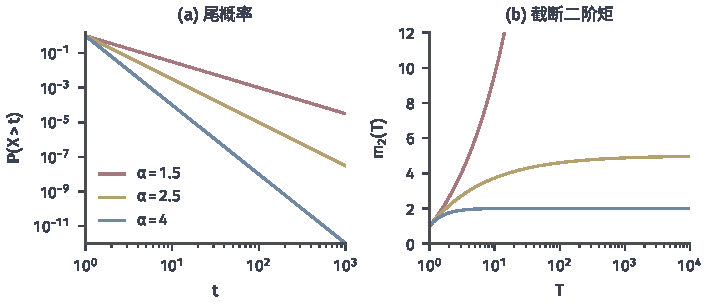
\includegraphics[width=120mm]{figures/02-abstract-mathematics/02-probability-spaces/matplotlib/pmod-moment-tails/figure.pdf}
  \caption{Pareto型尾部$\mathbb P(X>t)=t^{-\alpha}$（$t\ge1$），$\alpha=1.5,2.5,4$。(a) 双对数坐标下的尾概率，直线斜率为$-\alpha$；(b) 截断二阶矩$m_2(T)=\mathbb E[\min\{X,T\}^2]=1+2(T^{2-\alpha}-1)/(2-\alpha)$，横轴为对数尺度。$\alpha>2$时曲线收敛到$\mathbb EX^2=\alpha/(\alpha-2)$，$\alpha=1.5$时发散。}
  \label{fig:pmod-moment-tails}
\end{figure*}

\paragraph{Markov与Chebyshev不等式}
反过来，有限的矩可以控制尾概率。
这正是卷一Markov与Chebyshev不等式所做的事；它们只用到非负函数积分的单调性，所以在一般概率空间中原样成立。

\begin{theorem}[Markov与Chebyshev不等式]
\label{thm:pmod-markov}
设$X$是随机变量，$t>0$。
\begin{enumerate}
  \item 对任意$p>0$，$\mathbb P(|X|\ge t)\le\mathbb E|X|^p/t^p$。更一般地，若$h:[0,\infty)\to[0,\infty)$单调不减且$h(t)>0$，则$\mathbb P(|X|\ge t)\le\mathbb Eh(|X|)/h(t)$。
  \item 若$\mathbb EX^2<\infty$，则$\mathbb P(|X-\mathbb EX|\ge t)\le\operatorname{Var}X/t^2$。
\end{enumerate}
\end{theorem}

\begin{proof}
由$h$单调不减且非负，逐点有
$h(|X|)\ge h(t)\,\mathbb I_{\{|X|\ge t\}}$：$|X|\ge t$时右边为$h(t)\le h(|X|)$，否则右边为$0$。
对两边取期望，得$\mathbb Eh(|X|)\ge h(t)\,\mathbb P(|X|\ge t)$。
取$h(s)=s^p$得到\term{Markov不等式}（Markov inequality）的幂次形式；把$X$换成$X-\mathbb EX$并取$p=2$，得到\term{Chebyshev不等式}（Chebyshev inequality）。
\end{proof}

右边若为$+\infty$，不等式仍然成立，但不提供任何信息。
所以使用这些估计之前，必须先确认相应的矩有限；卷一在\BookChapterRef{chap:sampling-errors}{卷一“抽样分布与估计误差”章}中用它们证明了弱大数定律，后面的收敛章节也会以同样方式控制误差。

图~\ref{fig:pmod-markov-bounds}对$\alpha=3$的Pareto变量比较了三个矩界$\mathbb EX^p/t^p$与真实尾概率$t^{-3}$。
三个界都正确，但都远高于真实值：在$t=10$处，真实尾概率为$0.001$，$p=1,2,2.5$的界分别为$0.15$、$0.03$和约$0.019$。
阶数越高，界在大$t$处下降得越快；但常数$\mathbb EX^p=3/(3-p)$也越大，在$t=2$处$p=2.5$的界约为$1.06$，比平凡的上界$1$还差。
$p\ge3$时$\mathbb EX^p=\infty$，这一族界到此为止：矩界最多以多项式速度刻画尾部，系统的集中不等式留给\BookPartRef{part:inference-and-causal-identification}{卷四“推断与因果识别”部分}。

\begin{figure}[htbp]
  \centering
  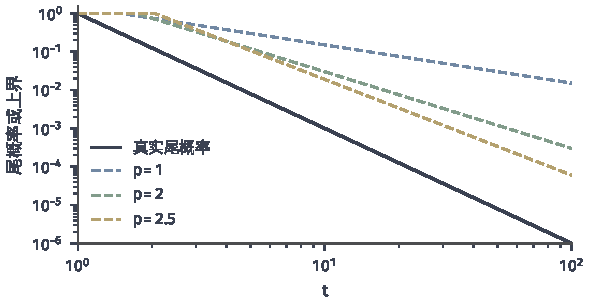
\includegraphics[width=100mm]{figures/02-abstract-mathematics/02-probability-spaces/matplotlib/pmod-markov-bounds/figure.pdf}
  \caption{$\alpha=3$的Pareto变量（$\mathbb P(X\ge t)=t^{-3}$，$t\ge1$）的真实尾概率（实线）与矩界$\min\{1,\mathbb EX^p/t^p\}$（虚线，$p=1,2,2.5$，$\mathbb EX^p=3/(3-p)$），双对数坐标。界始终在真实值之上；$p$越大，界在大$t$处越紧，在小$t$处可能更松。}
  \label{fig:pmod-markov-bounds}
\end{figure}

\subsection{随机向量的期望与协方差}

\paragraph{逐坐标的期望}
对随机向量$\bm X=(X_1,\dots,X_d)^\top$，若每个坐标可积，定义$\mathbb E\bm X=(\mathbb EX_1,\dots,\mathbb EX_d)^\top$；随机矩阵同样逐元素取期望。
坐标可积与范数可积是一回事：由
\[
  \max_i|x_i|\le\lVert\bm x\rVert_2\le\sum_{i=1}^d|x_i|,
\]
$\mathbb E\lVert\bm X\rVert_2<\infty$当且仅当每个$\mathbb E|X_i|<\infty$；有限维空间上各种范数彼此等价，选哪一种范数不影响结论。
期望的线性性逐坐标成立：对固定矩阵$\bm A$与向量$\bm b$，$\mathbb E[\bm A\bm X+\bm b]=\bm A\,\mathbb E\bm X+\bm b$，因为每个坐标都是有限个可积变量的线性组合。
这里只用到有限个实值积分，没有定义取值于一般Banach空间的随机对象的积分，也不需要函数空间的完备性。

\paragraph{乘积的可积性与Cauchy--Schwarz不等式}
协方差$\operatorname{Cov}(X,Y)=\mathbb E[(X-\mathbb EX)(Y-\mathbb EY)]$要求乘积可积。
由$2|xy|\le x^2+y^2$，$\mathbb EX^2$与$\mathbb EY^2$有限时$\mathbb E|XY|\le\tfrac12(\mathbb EX^2+\mathbb EY^2)<\infty$。
这个界还可以改进成乘积形式。

\begin{theorem}[Cauchy--Schwarz不等式]
\label{thm:pmod-cauchy-schwarz}
设随机变量$X,Y$满足$\mathbb EX^2<\infty$，$\mathbb EY^2<\infty$。则$XY$可积，且
\[
  \bigl(\mathbb E[XY]\bigr)^2\le\bigl(\mathbb E|XY|\bigr)^2\le\mathbb EX^2\,\mathbb EY^2.
\]
\end{theorem}

\begin{proof}
可积性已由上一段得到，第一个不等号是$|\mathbb E[XY]|\le\mathbb E|XY|$。
对实数$s$，展开非负随机变量的期望：
\[
  0\le\mathbb E\bigl(|X|-s|Y|\bigr)^2=\mathbb EX^2-2s\,\mathbb E|XY|+s^2\,\mathbb EY^2.
\]
若$\mathbb EY^2>0$，取$s=\mathbb E|XY|/\mathbb EY^2$，得$\mathbb EX^2-(\mathbb E|XY|)^2/\mathbb EY^2\ge0$，即所需结论。
若$\mathbb EY^2=0$，则$Y=0$几乎必然成立，$XY=0$几乎必然成立，两边都是$0$。
\end{proof}

取$X-\mathbb EX$与$Y-\mathbb EY$代入，得$|\operatorname{Cov}(X,Y)|\le\sqrt{\operatorname{Var}X\operatorname{Var}Y}$，所以有限二阶矩保证协方差有限；取$Y=1$，得$(\mathbb E|X|)^2\le\mathbb EX^2$。
这个不等式的思路与卷一用内积解释相关系数相同，这里补齐的是一般概率空间上的可积性。
本书称它为\term{Cauchy--Schwarz不等式}（Cauchy--Schwarz inequality），第~\ref{chap:conditional-expectation}章的条件均方误差和第~\ref{chap:weak-convergence-limit-theorems}章的多元极限都会使用它。

\paragraph{协方差矩阵的半正定性}
设$\mathbb E\lVert\bm X\rVert_2^2<\infty$，记$\bm\mu=\mathbb E\bm X$。
由上一段，每个$\operatorname{Cov}(X_i,X_j)$都有限，于是\term{协方差矩阵}（covariance matrix）
$\bm\Sigma=\mathbb E[(\bm X-\bm\mu)(\bm X-\bm\mu)^\top]$的每个元素都有定义。

\begin{theorem}[协方差矩阵半正定]
\label{thm:pmod-covariance-psd}
设$\bm X$是$d$维随机向量，$\mathbb E\lVert\bm X\rVert_2^2<\infty$。则对任意$\bm a\in\mathbb R^d$，
\[
  \bm a^\top\bm\Sigma\bm a=\operatorname{Var}(\bm a^\top\bm X)\ge0,
\]
因此$\bm\Sigma$是对称半正定矩阵。
\end{theorem}

\begin{proof}
$\bm a^\top\bm\Sigma\bm a=\sum_{i,j}a_ia_j\operatorname{Cov}(X_i,X_j)$，由期望对有限和的线性，这等于$\mathbb E\bigl[(\bm a^\top(\bm X-\bm\mu))^2\bigr]=\operatorname{Var}(\bm a^\top\bm X)$，非负。
对称性来自$\operatorname{Cov}(X_i,X_j)=\operatorname{Cov}(X_j,X_i)$。
\end{proof}

若某个$\bm a\ne\bm0$使$\bm a^\top\bm\Sigma\bm a=0$，则$\bm a^\top\bm X=\bm a^\top\bm\mu$几乎必然成立，$\bm X$几乎必然落在一个超平面内；协方差矩阵奇异并不违反任何定义。
定理把向量的二阶结构化为标量线性组合的方差，这是后面处理多元极限时的基本桥梁。
高斯向量协方差的具体计算见\BookChapterRef{chap:random-vectors}{卷一“随机向量与联合分布”章}，这里不再重复。

\subsection{凸函数与期望}

\paragraph{支撑直线与Jensen不等式}
先求平均再作非线性变换，与先变换再求平均，结果一般不同。
方差非负就是一个例子：$\mathbb EX^2-(\mathbb EX)^2=\operatorname{Var}X\ge0$，即$(\mathbb EX)^2\le\mathbb EX^2$。
对一般的凸函数，这种比较称为\term{Jensen不等式}（Jensen's inequality），比较的依据是\term{支撑直线}（supporting line）。

设$\varphi:\mathbb R\to\mathbb R$是\term{凸函数}（convex function）。
凸性使差商$(\varphi(x)-\varphi(m))/(x-m)$随$x$单调不减，所以右导数$c=\varphi'_+(m)$存在且有限；对$x>m$，差商不小于$c$，对$x<m$，差商不大于左导数$\varphi'_-(m)\le c$。
两种情形都给出
\begin{equation}
  \varphi(x)\ge\varphi(m)+c(x-m),\qquad x\in\mathbb R,
  \label{eq:pmod-support-line}
\end{equation}
即直线$\ell(x)=\varphi(m)+c(x-m)$在$m$处接触$\varphi$的图像，并处处位于图像下方。
有限凸函数是连续的，因而Borel可测，$\varphi(X)$是随机变量。

\begin{theorem}[Jensen不等式]
\label{thm:pmod-jensen}
设$X$是可积随机变量，$\varphi:\mathbb R\to\mathbb R$是凸函数。
则$\varphi(X)^-$可积，$\mathbb E\varphi(X)$在$(-\infty,+\infty]$中有定义，并且
\[
  \varphi(\mathbb EX)\le\mathbb E\varphi(X).
\]
\end{theorem}

\begin{proof}
取$m=\mathbb EX$，$\ell$为式~\eqref{eq:pmod-support-line}中的支撑直线，则逐点有$\varphi(X)\ge\ell(X)$。
于是$\varphi(X)^-\le\ell(X)^-\le|\varphi(m)|+|c|\,|X-m|$，右边可积，所以$\varphi(X)^-$可积，$\mathbb E\varphi(X)$有定义（可能为$+\infty$）。
由于$\varphi(X)-\ell(X)\ge0$且$\ell(X)$可积，
\[
  \mathbb E\varphi(X)\ge\mathbb E\ell(X)=\varphi(m)+c(\mathbb EX-m)=\varphi(\mathbb EX).
\]
\end{proof}

证明中先确认负部可积这一步不能省：否则$\mathbb E\varphi(X)$可能是未定义的$\infty-\infty$，比较大小无从谈起。
图~\ref{fig:pmod-jensen-support}以三点分布说明证明的几何含义。
$X$取$-1,0.5,2$，概率$0.3,0.5,0.2$，均值$\mu=0.35$。
支撑直线在$\mu$处接触$\varphi(x)=e^x$，直线上三点的加权平均恰好落回$\varphi(\mu)=e^{0.35}\approx1.42$；曲线上三点的加权平均$\mu_\varphi=\mathbb Ee^X\approx2.41$。
两者之差是曲线与支撑直线在各取值处竖直距离的加权平均。

\begin{figure}[htbp]
  \centering
  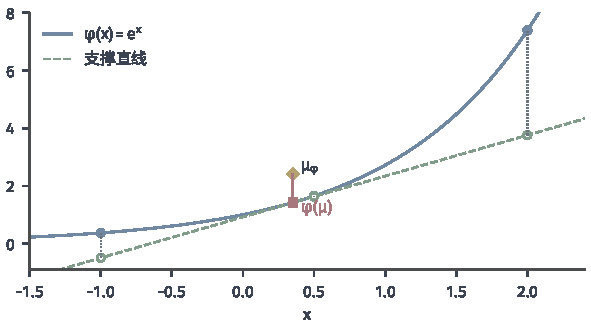
\includegraphics[width=100mm]{figures/02-abstract-mathematics/02-probability-spaces/matplotlib/pmod-jensen-support/figure.pdf}
  \caption{Jensen不等式的支撑直线论证。$X$取$-1,0.5,2$的概率分别为$0.3,0.5,0.2$，$\mu=\mathbb EX=0.35$。实线为$\varphi(x)=e^x$，虚线为它在$\mu$处的切线（支撑直线）。实心点为$(x_i,\varphi(x_i))$，空心点为直线上的对应点，点线为两者的竖直差距。方块为$\varphi(\mu)\approx1.42$，菱形为$\mu_\varphi=\mathbb E\varphi(X)\approx2.41$。}
  \label{fig:pmod-jensen-support}
\end{figure}

\paragraph{绝对值、幂次与等号条件}
取$\varphi(x)=|x|$得$|\mathbb EX|\le\mathbb E|X|$；取$\varphi(x)=|x|^p$（$p\ge1$）得$|\mathbb EX|^p\le\mathbb E|X|^p$。
Jensen不等式还给出定理~\ref{thm:pmod-moment-monotone}的精细版本。
设$0<p<q$且$\mathbb E|X|^q<\infty$；由该定理$Y=|X|^p$可积，对凸函数$\varphi(y)=|y|^{q/p}$应用Jensen不等式，得
\[
  \bigl(\mathbb E|X|^p\bigr)^{q/p}\le\mathbb E|X|^q,\qquad\text{即}\qquad
  \bigl(\mathbb E|X|^p\bigr)^{1/p}\le\bigl(\mathbb E|X|^q\bigr)^{1/q}.
\]
在概率空间上，$p\mapsto(\mathbb E|X|^p)^{1/p}$单调不减：阶数越高，这种“平均大小”越不会变小。这一步用到总质量为$1$，对一般测度并不成立。

等号何时成立？
若$\varphi$严格凸，则支撑直线只在$m$处接触图像，$x\ne m$时$\varphi(x)>\ell(x)$。
当$\mathbb E\varphi(X)=\varphi(\mathbb EX)$且有限时，非负变量$\varphi(X)-\ell(X)$的期望为零，因此几乎必然为零，从而$X=\mathbb EX$几乎必然成立：严格凸函数的等号只属于几乎必然为常数的变量。
$|x|$不是严格凸的，它的等号条件更宽：$|\mathbb EX|=\mathbb E|X|$当且仅当$X$几乎必然不变号。
例如$\mathbb EX\ge0$时，等式意味着$\mathbb E(|X|-X)=0$，而$|X|-X\ge0$，所以$|X|=X$几乎必然成立。
给定部分信息后的条件版本是第~\ref{chap:conditional-expectation}章的定理~\ref{thm:cond-jensen}。

\section{本章小结}
\label{sec:pmod-summary}

本章把概率计算分成三个层次。
第一层是概率空间上的随机对象：$(\Omega,\mathcal F,\mathbb P)$给出可能结果、允许判断的事件及其概率，随机对象是可测映射，它生成的$\sigma(X)$说明观测能分辨哪些事件。

第二层是取值空间上的分布：$P_X=X_\#\mathbb P$只保留各取值集合上的概率，舍弃了“哪个结果给出哪个值”，所以同分布的变量可以处处不相等，相同边缘的随机变量列可以有完全不同的样本轨迹。
多个对象一起出现的规律由联合分布记录，边缘分布只是它的投影；独立性要求联合分布恰好分解为边缘的乘积测度，这一条件只需在生成族上核对，并在不相交的分组与可测变换后保持。

第三层是对分布的累计：期望是对$\mathbb P$的积分，又可以通过分布积分公式在取值空间上计算，因而点质量、密度和两者的混合都用同一个公式处理；矩条件记录尾部累计的可积程度，Markov、Cauchy--Schwarz与Jensen不等式在相应矩有限时控制尾概率、乘积与非线性变换。

回到章首的问题。
三位骰子记录员面对同一个概率空间，区别在于各自记录生成的$\sigma$代数；有空闲窗口的等待时间可以直接对混合分布积分，得到$\mathbb EX=0.6$；同分布与相同边缘都只描述取值空间上的规律，不能决定样本点上的相等、收敛或共同发生。
不过，现在我们只能说清“已知的信息是什么”，还不能在只掌握部分信息时给出保持正确累计的平均值，例如只知道点数和时，第一枚骰子的平均点数应当是多少。
第~\ref{chap:conditional-expectation}章由此建立条件期望与条件分布；随后两章分别研究同一概率空间上随机变量列的收敛，以及只比较取值空间上分布的弱收敛，本章区分的样本点与分布两个层次将在那里分别成为两类收敛的出发点。
